\documentclass{standalone}
\usepackage{tikz}
\usepackage{mtpro2}
\usetikzlibrary{calc,patterns,decorations.pathmorphing,decorations.markings}

\begin{document}
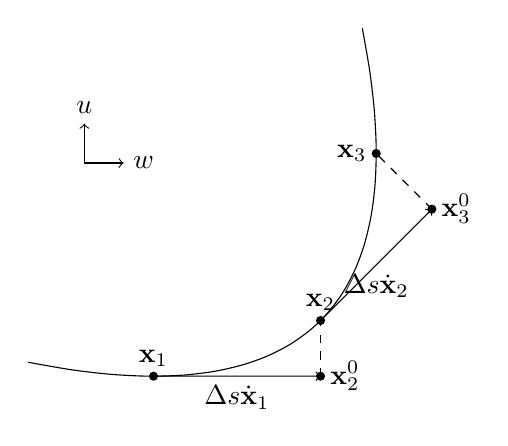
\begin{tikzpicture}
\begin{scope}[rotate=45]
% -- define nodes
\coordinate (x1) at (-2,1);
\coordinate (x2) at (0,0);
\coordinate (x20) at (-.5,-.5);
\coordinate (x3) at (2,1);
\coordinate (x30) at (2,0);
\draw[fill] (x1) circle (.05) node[above]{$\mathbf x_1$};
\draw[fill] (x2) circle (.05) node[above]{$\mathbf x_2$};
\draw[fill] (x20) circle (.05) node[right]{$\mathbf x_2^0$};
\draw[fill] (x3) circle (.05) node[left]{$\mathbf x_3$};
\draw[fill] (x30) circle (.05) node[right]{$\mathbf x_3^0$};
% -- draw curve
\draw [smooth,samples=20,domain=-3:3] plot(\x,{\x*\x/4});
% -- draw lines
\draw [->] (x1)-- node[below]{$\Delta s \dot{\mathbf x}_1$} (x20) ;
\draw [dashed] (x20)-- (x2) ;
\draw [->] (x2)-- node[below]{$\Delta s \dot{\mathbf x}_2$} (x30) ;
\draw [dashed] (x30)-- (x3) ;
\end{scope}
% -- draw coordinates
\draw [->] (-3,2)-- ++(.5,0) node[right]{$w$} ;
\draw [->] (-3,2)-- ++(0,.5) node[above]{$u$} ;
\end{tikzpicture}
\end{document}